\subsection{Elektronik}
Zur Übersicht der verwendeten Elektronik Hardware dient das Blockschaltbild Abb. \ref{fig:Blockschaltbild_Komponenten}. Es bildet eine Auflistung sämtlicher Elektronik Komponenten, welche in Blöcke zusammengefasst sind. Detaillierte Angaben zu den jeweiligen Komponenten, sowie Schaltungen finden sich in den Kapiteln \ref{kap:Evaluation_der_Komponenten} und \ref{kap:Umsetzung}. 


\begin{figure}[H]
	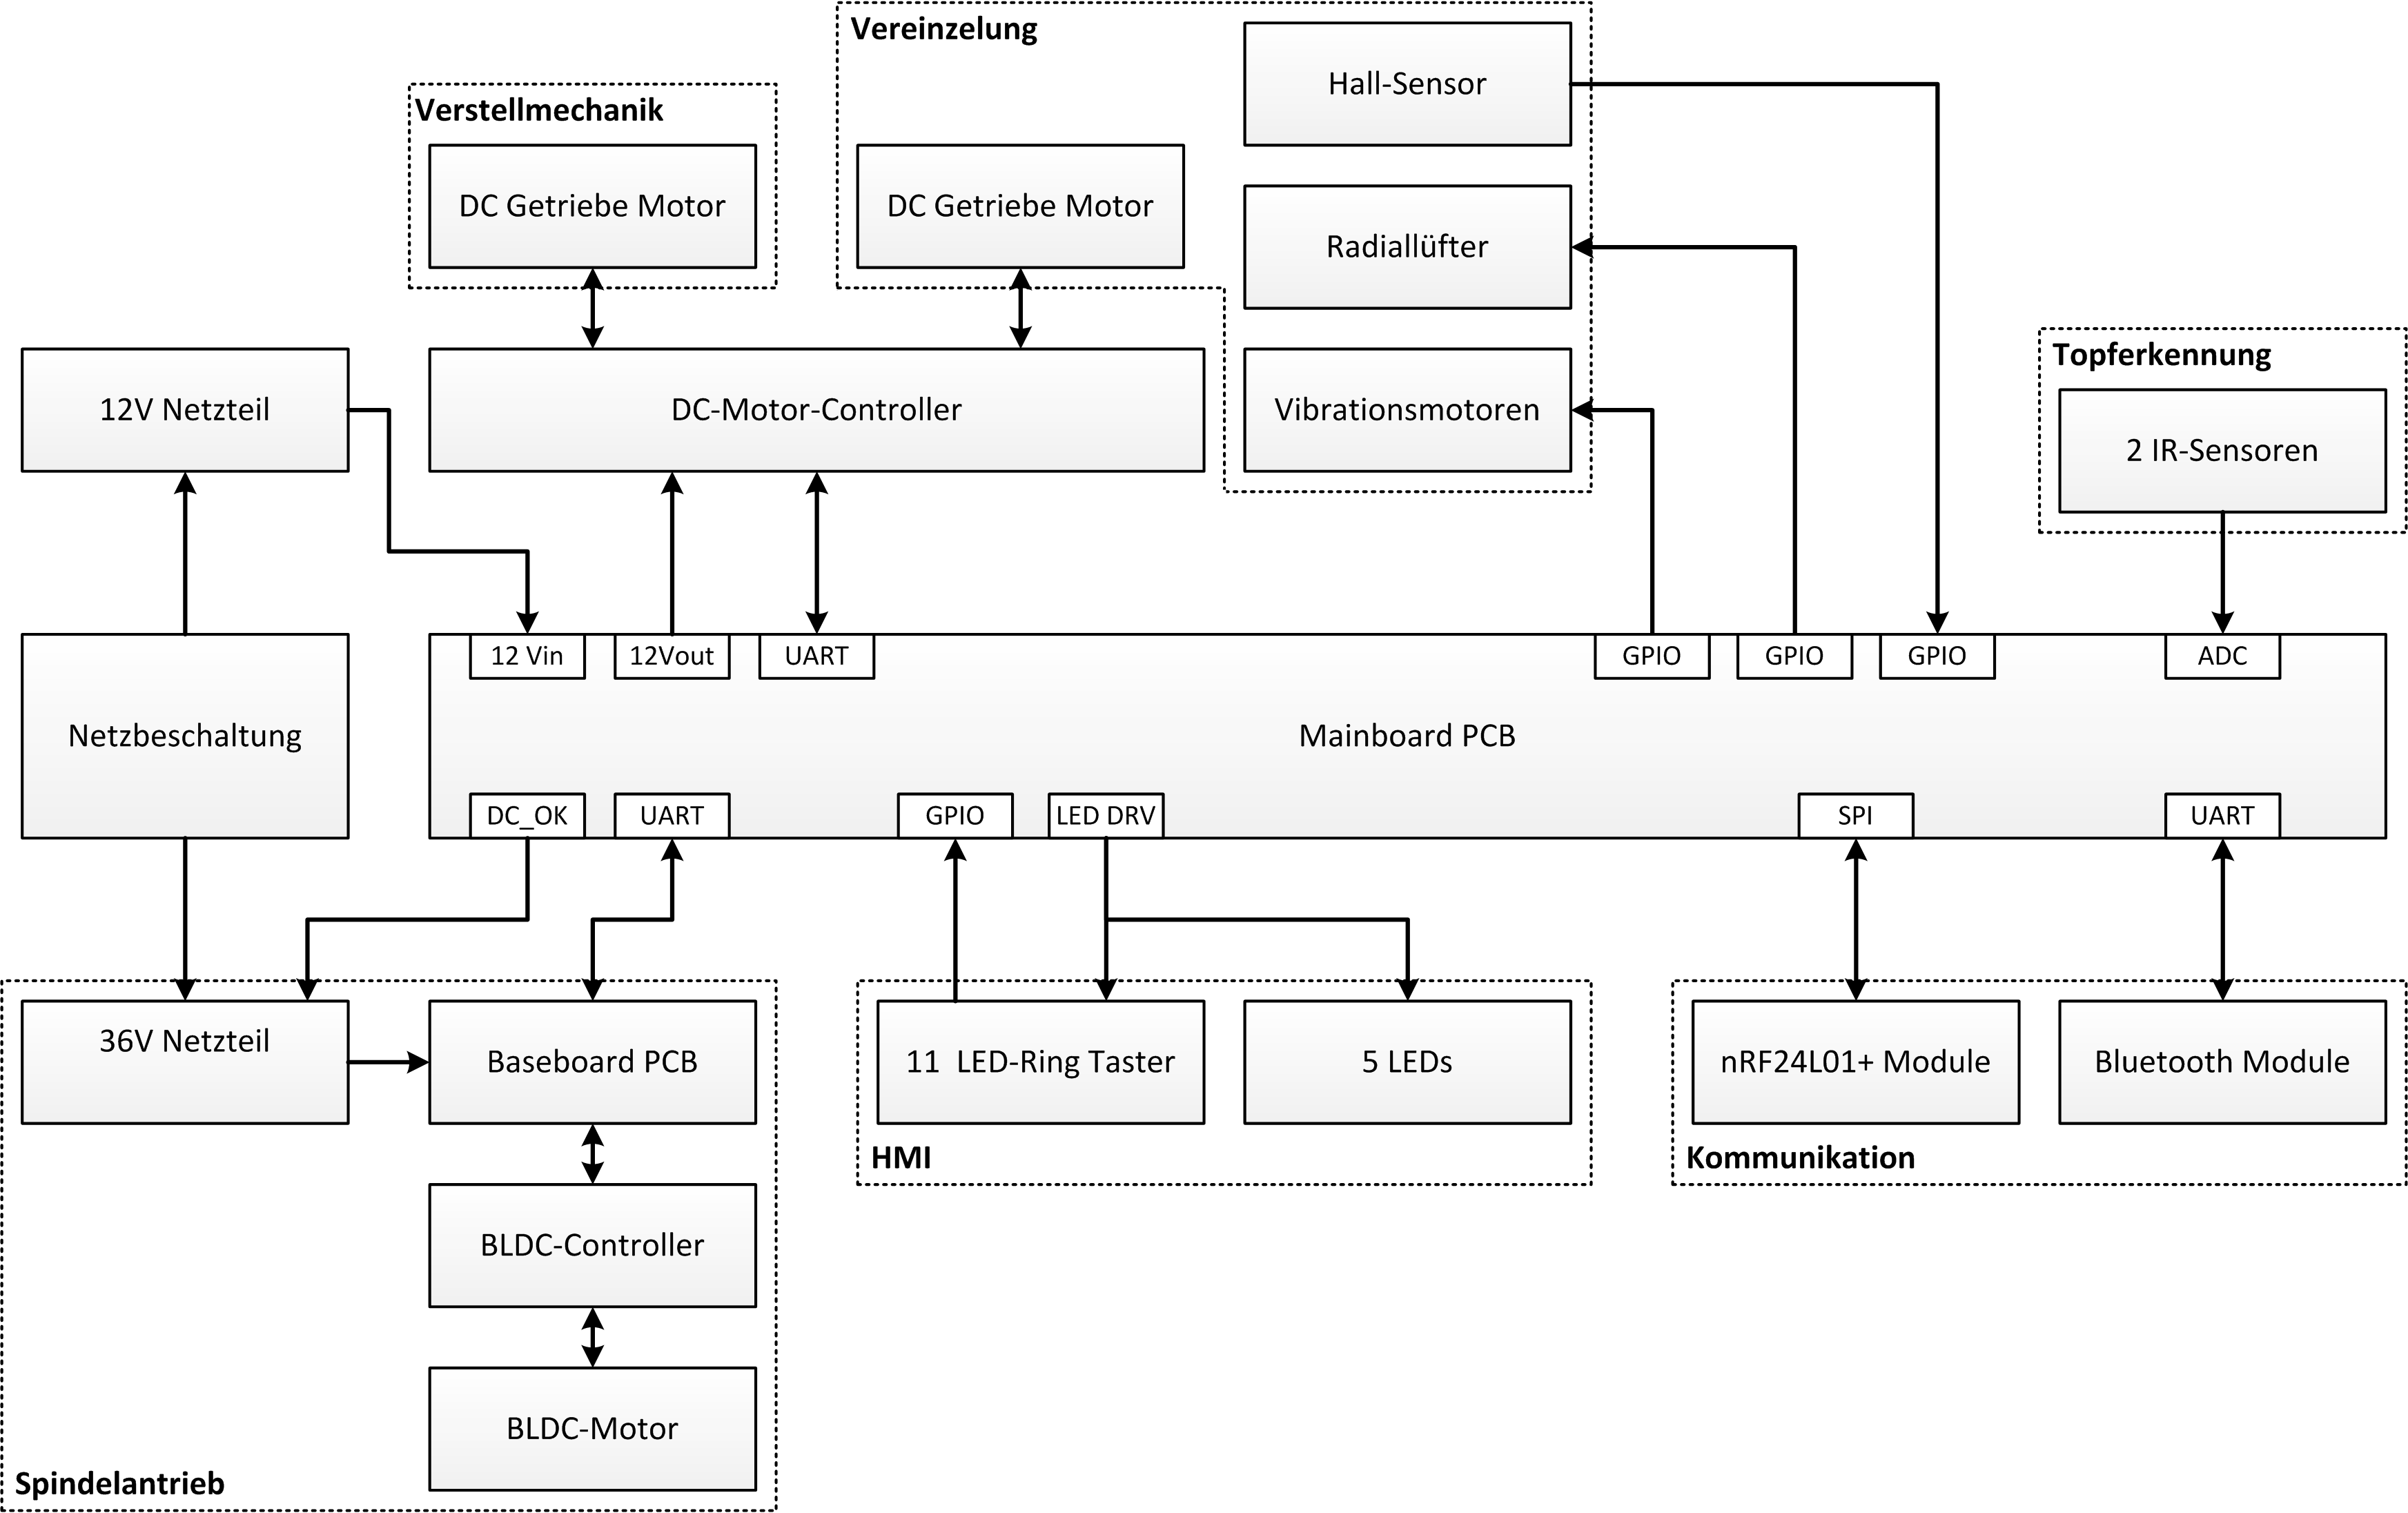
\includegraphics[width=1\textwidth]{Illustrationen/5-Konzept/Blockschaltbild_Komponenten.png}
	\caption{Blockschaltbild der Elektronik Komponenten}
	\label{fig:Blockschaltbild_Komponenten}
\end{figure}

Im folgenden Abschnitt werden die Blöcke das Blockschaltbild kurz erläutert:
\begin{itemize}
	\item \textbf{Netzbeschaltung:} Gemäss Pflichtenheft, soll der Planting Robot über 230V Netzspannung betrieben werden können. Diese Anforderung setzt eine adäquate Schutzschaltung voraus. So wurde ein Leitungsschutzschalter, sowie eine Relais Selbsthalteschaltung zum Ein und Ausschalten der Anlage über zwei Taster mit Betriebsanzeige vorgesehen. Des weiteren wurde das Alu Blech, auf welches die Netzkomponenten befestigt wurden, mit dem Schutzleiter verbunden.

	\item \textbf{36V Netzteil:} Um die hohe Leistungsanforderung an den Spindelantrieb bei moderatem Stromfluss erfüllen zu können, wird dessen Motor mit einem 36V Netzteil gespeist. Das FRDM-Board kann über das enable Signal des Netzteils die 36V Ausgangsspannung ein- und ausschalten.
	
	\item \textbf{Baseboard PCB:} Als Schnittstelle zwischen Mainboard PCB und BLDC-Controller dient das Baseboard PCB. Es vereinfacht die Verkabelung mit dem BLDC-Controller Board und verfügt über Drehpotentiometer zur schnellen Inbetriebnahme des BLDC-Motors.
	
	\item \textbf{BLDC-Controller:} Der BLDC-Controller wird über einen UART Port des FRDM-Boards angesteuert. Mit Hilfe der Hall-Sensor Auswertung des BLDC-Controllers kann der BLDC-Motor als Servomotor mit Positionsregelung betrieben werden. Damit kann ein Maximum an Präzision und Geschwindigkeit bei der Ansteuerung des Spindelantriebs garantiert werden.
	
	\item \textbf{Spindelantrieb:} Der Motor für den Spindelantrieb muss fähig sein, die Hubspindel in sehr kurzer Zeit auf Nenndrehzahl zu beschleunigen und wieder bis zum Stillstand zu verzögern. Benötigt wird deshalb ein Motor, welcher ein hohes Anlaufdrehmoment zur Verfügung stellt und häufigen Lastwechseln dauerhaft standhält. Dafür geeignet ist ein BLDC Motor mit Hall-Sensoren.
		
	\item \textbf{HMI:} Das Human-Machine Interface soll gemäss Pflichtenheft möglichst simpel gehalten werden. Es besteht deshalb aus Tastern zur Befehlseingabe und LEDs zur Statusanzeige. 
		
	\item \textbf{Topferkennung:} Die Topferkennung übernimmt zwei Funktionen. Zum einen ist sie für das Timing des Setzprozesses verantwortlich indem sie erkennt, ob sich ein Topf vor dem Planting Robot im Stillstand befindet und so bereit für den Setzprozess ist. Zum anderen soll sie im Umfang der Wunschanforderungen die Topfgrösse bestimmen und dementsprechend die Verstellmechanik konfigurieren können.
	
	\item \textbf{Kommunikation:} Zur Erleichterung der Inbetriebnahme sollen Parameter des Programms auf dem Mikrocontroller Board zur Laufzeit verändert werden können. Dies kann über ein Konsolenprogramm am Computer, welcher über Bluetooth mit dem Mikrocontroller Board verbunden ist, realisiert werden. Oder über das Funkmodul nRF24L01+ mit welchem ein zweites Mikrocontroller Board angesprochen werden kann.
			
	\item \textbf{12V Netzteil:} Um einen sicheren Betrieb der Elektronik während hohen Leistungsspitzen des Spindelantriebs zu garantieren, wird diese über ein separates Netzteil versorgt. Des weiteren werden auch die kleineren DC Getriebemotoren über dieses Netzteil gespeist. Das 12V Netzteil wird über das Zuschalten der Netzspannung gesteuert und kann nicht über den Mikrocontroller geschaltet werden.
	
	\item \textbf{DC-Motor-Controller:} Um die beiden DC-Getriebemotoren anzusteuern wird ein 2 Kanal Motorentreiber verwendet. Dieser ist, wie der BLDC-Controller, in der Lage mit Hilfe der Quadratur Encoder Signale der Motoren, eine Positionsregelung auszuführen. Der Treiber wird über UART angesteuert. Weiter befindet sich auf dem Motorcontroller eine 5V Speisung welche auf das Mainboard geführt ist. Dieses Spannungspotential wird auf dem Mainboard für den Antrieb von allfälligen Servos verwendet.
	
	\item \textbf{Verstellmechanik:} Die Verstellmechanik kann den Radius der Stechdornen und somit der Setzlöcher verändern. Für den Antrieb dieser Einheit kommt ein DC-Getriebemotor mit Encoder zum Einsatz. Dieser Motor wird über die Positionsregelung des DC-Motor-Controllers angesteuert. Zur absoluten Positionsbestimmung während der Initialisierung fährt der Motor an den Anschlag der Verstellmechanik bis ein definierter Laststrom erreicht wird.
	
	\item \textbf{Vereinzelung:} Die Drehscheibe der Vereinzelung wird in einer Dreh/Stopp Bewegung angetrieben. Das heisst, sie dreht sich jeweils so weit bis die Löcher der Lochmasken übereinstimmen. Zu diesem Zeitpunkt wird die Drehscheibe gestoppt und die Nemacaps können durch die Löcher fallen. Wie in der Verstellmechanik wird ein DC-Getriebemotor mit Encoder für den Antrieb der Vereinzelung verwendet. Zur absoluten Positionsbestimmung kommt ein Hall Sensor zum Einsatz, welcher einen Stabmagnet auf der Drehscheibe erkennt. Um allfälligen Verstopfungen der Vereinzelung vorzubeugen werden mehrere Vibrationsmotoren an der Mechanik angebracht.
	
	\item \textbf{Mainboard PCB:} Wie im Blockschaltbild dargestellt werden sämtliche Elektronikkomponenten über das selbst entwickelte Mainboard PCB miteinander verknüpft. Auf dem Mainboard PCB befindet sich das Mikrocontroller Board FRDM-KL25Z, auf welchem ein RTOS mit entsprechender Software gemäss Kap. \ref{kap:Software} implementiert ist.
\end{itemize}